\documentclass[11pt]{article}






%\usepackage{times}
\usepackage{palatino}%charter}
\usepackage{wrapfig}
\usepackage{citesort}
\usepackage{epsfig}
\usepackage{graphicx}
\usepackage{color}
\usepackage{fullpage}
\usepackage{amssymb}
\usepackage{amsmath}
\usepackage{theorem}
%\theoremstyle{remark} 
%\theoremstyle{definition}
%\usepackage{wide}
%\usepackage[ruled, vlined]{algorithm2e}
\usepackage[ruled, vlined, linesnumbered]{algorithm2e}
\usepackage{color}



\newcommand{\veps}{\varepsilon}
\newcommand{\eps}{\epsilon}
\newcommand{\E}{\mathbf{E}}
\renewcommand{\Pr}{\mathbf{Pr}}
\newcommand{\abs}[1]{\left| #1 \right|}
\newcommand{\norm}[1]{\left\lVert #1 \right\rVert}

\newcommand{\bbR}{\mathbb{R}}
\newcommand{\bbZ}{\mathbb{Z}}
\newcommand{\calC}{\mathcal{C}}
\newcommand{\emRed}[1][]{\textcolor{red} #1}


\newtheorem{theorem}{Theorem}
\newtheorem{protocol}{Protocol}
\newtheorem{lemma}{Lemma}
\newtheorem{claim}{Claim}
\newtheorem{property}{Property}
\newtheorem{fact}{Fact}
\newtheorem{observation}{Observation}
\newtheorem{heuristic}{Heuristic}
\newtheorem{solution}{Solution}
\newtheorem{corollary}{Corollary}
\newtheorem{scheme}{Scheme}
\newtheorem{strategy}{Strategy}
\newtheorem{invariant}{Invariant}
{\theorembodyfont{\rmfamily}
\newtheorem{remark}{Remark}}
{\theorembodyfont{\rmfamily}
\newtheorem{definition}{Definition}}



\newcommand{\chensays}[2][]{\textcolor{red} {\textsc{Chen #1:} \emph{#2}}}




\newenvironment{proof}{\trivlist\item[]\emph{Proof:}}%
{\unskip\nobreak\hskip 1em plus 1fil\nobreak$\Box$
\parfillskip=0pt%
\endtrivlist}





\begin{document}

\title{A Survey on \\ Distributed/Streaming Submodular Optimization}
\author{Jiecao Chen}
\date{\today}

\maketitle
%\tableofcontents
\section{Introduction}
Submodularity is a property of set functions with deep theoretical and practical consequences. Submodular functions occur in a variety of applications, including representative skyline selection \cite{SLN+11}, network structure learning \cite{GLK10}, influence maximization \cite{KKT03}, document summarization \cite{LB11}, image segmentation \cite{BJM01,KKT09} and many others.


There is a large body of research in submodular optimization which we can not cover thoroughly here. In this survey, we focus on the recent advances in optimizing (mostly, maximizing) submodular functions in distributed and streaming setting.



Through Lov{\'a}sz' extension, a submodular minimization problem can be solved via techniques from convex optimization. Therefore most work focuses on submodular maximization. In particular, almost all results for distributed and streaming submodular optimization are for maximization problems. In this survey, we also focus on submodular maximization, but will briefly mention minimization problems as well when necessary.

\subsection{Notations}
Through out this survey, 

we use $V$ to represent the ground set we consider. 

$2^V$ is the power set of $V$ (i.e. the set of all subsets of $V$).

In general, $A^V$ is the collection of maps from $V$ to $A$. 

For simplicity, we sometime write $A \cup \{x\}$ as $A + x$.


\section{Submodularity}
In this section, we first give several equivalent definitions of submodularity, and then we introduce several fundamental properties of submodular functions. We also discuss various constraints that occur frequently in submodular optimization problems. In the last part of this section, we cover algorithms that solve constrained submodular maximization problems with theoretical approximation guarantee. 

\subsection{Definitions}
There are many equivalent definitions, and we will discuss three of them in this section. 

\begin{definition}[submodular concave]
  \label{def:sub-concave}
  A function $f:~2^V \rightarrow \bbR$ is \emRed{submodular} if for any $A, B \subseteq V$, we have that:
  \begin{equation}
    \label{eq:sub-concave}
    f(A) + f(B) \geq f(A \cup B) + f(A \cap B).
  \end{equation}
\end{definition}

An alternate equivalent definition is more interpretable in many situations,

\begin{definition}[diminishing returns]
  \label{def:sub-diminishing}
  A function $f: 2^V \rightarrow \bbR$ is \emRed{submodular} if for any $A \subseteq B \subset V$, and $v \in V\backslash B$, we have that:
  \begin{equation}
    \label{eq:sub-diminishing}
    f(A + v) - f(A) \geq f(B + v) - f(B).
  \end{equation}
\end{definition}

Intuitively, this definition requires that the incremental ``gain'' of adding a new element $v$ decreases (diminishes) as the base set grows from $A$ to $B$. We will see that this property is actually shared by many real-world phenomenons.

It turns out that a stronger but equivalent statement can also serve as the definition of a submodular function,

\begin{definition}[group diminishing returns]
  \label{def:sub-diminishing-group}
  A function $f: 2^V \rightarrow \bbR$ is \emRed{submodular} if for any $A \subseteq B \subset V$, and $C \subseteq V\backslash B$, we have that:
  \begin{equation}
    \label{eq:sub-diminishing-group}
    f(A \cup C) - f(A) \geq f(B \cup C) - f(B).
  \end{equation}
\end{definition}


\subsection{Modularity and Supermodularity}
We also briefly mention modularity and supermodularity here. These two concepts are closely related to submodularity. 

A function $f: 2^V \rightarrow \bbR$ is modular if we replace inequality by equality in Definition \ref{def:sub-diminishing} (or any of other two). Formally, 

\begin{definition}[Modularity]
  \label{def:modular}
  A function $f: 2^V \rightarrow \bbR$ is \emRed{modular} if for any $A \subseteq B \subset V$, and $v \in V\backslash B$, we have that:
  \begin{equation}
    \label{eq:modular}
    f(A + v) - f(A) = f(B + v) - f(B).
  \end{equation}
\end{definition}
Notably, a modular function $f$ can always be written as
$$f(S) = f(\emptyset) + \sum_{v\in S} \left( f(\{v\}) - f(\emptyset) \right)$$
for any $S \subseteq V$.

If we further assume $f(\emptyset) = 0$ (in this case, we call $f$ \emRed{normalized}), we have a simplified expression,

$$f(S) = \sum_{v\in S} f(\{v\}).$$


Modularity can be useful in our discussion of submodularity, because one can use modular functions to construct submodular functions with desired properties in their applications. Examples can be found in e.g. \cite{LB11,LB11word}.




A supermodular function is defined by flipping the inequality sign in the definition of a submodular function. Formally,
\begin{definition}[Supermodularity]
  \label{def:supermodular}
  A function $f: 2^V \rightarrow \bbR$ is \emRed{modular} if for any $A \subseteq B \subset V$, and $v \in V\backslash B$, we have that:
  \begin{equation}
    \label{eq:submodular}
    f(A + v) - f(A) \leq f(B + v) - f(B).
  \end{equation}
\end{definition}

We will focus on submodular functions because a function is supermodular if and only if its negative is submodular. 



\subsection{Properties}
Like convex and concave functions, submodular functions have many nice properties. Lov{\'a}sz's description of convex functions \cite{L83} can be viewed as accurate comments on submodularity:
\begin{quote}
 - Convex functions occur in many mathematical models in economy,
engineering, and other sciences. Convexity is a very natural property
of various functions and domains occurring in such models; quite
often the only non-trivial property which can be stated in general.

- Convexity is preserved under many natural operations and
transformations, and thereby the effective range of results can be
extended, elegant proof techniques can be developed as well as
unforeseen applications of certain results can be given.

- Convex functions and domains exhibit sufficient structure so that a
mathematically beautiful and practically useful theory can be
developed.

- There are theoretically and practically (reasonably) efficient methods
to find the minimum of a convex function.
\end{quote}

We survey several useful properties which can be useful in our later section. More properties of submodularity can be found in e.g. \cite{B14,F05}.





Submodularity is close under addition,
\begin{property}
  \label{prop:addition}
  Let $f_1, f_2: 2^V \rightarrow \bbR$ be two submodular functions. Then 
  $$f: 2^V\rightarrow \bbR~{with}~ f(A) = \alpha f_1(A) + \beta f_2(A)$$ 
is submodular for any fixed $\alpha, \beta \in \bbR^+$.
\end{property}


Adding a modular function does not break submodularity,
\begin{property}
  \label{prop:modular}
  Let $f_1, f_2: 2^V \rightarrow \bbR$, $f_1$ is submodular and $f_2$ is modular. Then
  $$f: 2^V \rightarrow \bbR~\text{with}~ f(A) = f_1(A) + \alpha f_2(A)$$
is submodular for any fixed $\alpha \in \bbR$.
\end{property}

Submodularity is preserved under restriction,
\begin{property}
  \label{prop:restriction}
  Let $f: 2^V \rightarrow \bbR$ be a submodular function. Let $S\subseteq V$ be a fixed set. Then
$$f':2^V \rightarrow \bbR~{with}~f'(A) = f(A\cap S)$$
is submodular.
\end{property}

As a direct implication of Property \ref{prop:addition} and Property \ref{prop:restriction}, we have the following more general result,
\begin{property}
Let $f:2^V \rightarrow \bbR$ be a submodular function, $\calC = \{C_1, C_2, \ldots, C_k\}$ be a collection of subsets of $V$ (i.e. each $C_i \subseteq V$). Then
$$f':2^V \rightarrow \bbR~{with}~f'(A) = \sum_{C\in\calC}f(A\cap C)$$ 
is submodular.
\end{property}
This property can be useful in graphical models and image processing. \chensays{TODO: show examples}


Following property can be useful when we show that the objective function of k-medoid problem is supermodular,
\begin{property}
  \label{prop:max}
Consider $V$ as a set of indices. Let $\mathbf{c}\in \bbR^V$ be a fixed vector, $c_i$ be its $i$th coordinate. Then 
$$f:2^V \rightarrow \bbR~{with}~ f(A) = \max_{j\in A}c_i$$ 
is submodular.
\end{property}

We can use non-negative modular function and a concave function to construct submodular functions,
\begin{property}
  Let $m: 2^V \rightarrow \bbR^+$ be a modular function, and $f$ a concave function over $\bbR$. Then
$$f: 2^V \rightarrow \bbR ~{with}~ f(A) = g(m(A))$$
is submodular.
\end{property}

Before introducing the next property, we define the monotonitcity of set function,
\begin{definition}[Monotonitcity]
  An set function $f: 2^V \rightarrow  \bbR$ is said to be non-decreasing if for any $A\subseteq B \subseteq V$, $f(A) \leq f(B)$. Non-increasing set functions are defined in similar way.
\end{definition}
When we say a submodular function is monotone, we mean it is non-decreasing.

\begin{property}
  Let $f, g: 2^V \rightarrow \bbR$ be two submodular functions. If $(f - g)(\cdot)$ is either non-decreasing or non-increasing, then $f: 2^V \rightarrow \bbR$ with
$$f(A) = \min(f(A), g(A))$$
is submodular.
\end{property}



\subsection{Constraints}
Now we discuss the constraints in submodular optimization problems. A submodular maximization problem usually has the following form,
\begin{equation}
  \label{eq:optimization}
  \argmax_{I\in\calI} f(I)
\end{equation}

where $f$ is a submodular function and $\calI \subseteq 2^V$ is the collection of all feasible solutions. We call $\calI$ the \emRed{constraint} of the optimization problem. The structure of $\calI$ plays a crucial role in submodular optimization. Different constraints have different hardness results, normally the difficulty increases when the constraint becomes more general. We will introduce cardinality constraint, knapsack constraint, matroid, and p-matchoid.

\subsubsection{Cardinality Constraint}
Cardinality constraint is perhaps the most straightforward constraint we would discuss in this survey. Efficient algorithms have been developed for finding or approximating the optimal solution of (\ref{eq:optimization}). There are also a lot of discussions on optimization subject to cardinality constraint, in both streaming and distributed setting. 

A \emRed{cardinality constraint} is parameterized with a fixed constant $k \in \bbZ^+$. It is simply defined as $\calI = \{A \subseteq V ~|~ |V| \leq k\}$, i.e. all subsets of $V$ with size no larger than $k$. Cardinality constraint is arguably the most popular constraint, and it occurs everywhere. For example, in k-medoid clustering, we want to find a set $S$ of \emph{at most} $k$ points, that minimizes the total distance of all points to $S$.  

\subsubsection{Knapsack Constraint}
Knapsack constraint generalizes cardinality constraint by assigning each element in $V$ a weight. Given a budget $W > 0$ and assume that each $i \in V$ is assigned a weight $w_i \geq 0$, a \emRed{knapsack constraint} can be defined as $\calI = \{S \subseteq V ~|~ \sum_{i\in S} w_i \leq W \}$.


\subsubsection{Matroid}
Informally,  \emRed{matroid} is the abstraction of the \emph{independence} concept in linear algebra. In fact there are so many results around Matroid and the Matroid itself becomes a subfield of algebra. We cover some basics of Matroid theory and from which readers can easily see how powerful this concept is. 

Before discussing the concept of a matroid, we briefly review the independence concept from linear algebra. For simplicity, let us just consider $\bbR^d$ instead of a general linear space. A subset $S$ of $\bbR^d$ is said to be \emph{independent} if there does not exist any $\mathbf{x}\in S$ such that $\mathbf{x}$ can be represented by linear combination of vectors in $S\backslash\{\mathbf{x}\}$. 

Let $\calI = \{S \subseteq \bbR^d~|~S ~\text{is independent}~\}$, i.e. only a independent set can be considered feasible. From what we learn in college linear algebra course, we know $\calI$ has the following propertie: 1) $\emptyset \in \calI$; 2) if $I\in \calI$, any of $I$'s subsets is also in $\calI$ (or equivalently, $\calI$ is \emRed{hereditary}); 3) if $J, I\in \calI$ and $J$ has smaller size than $I$, we must be able to find an element  $\mathbf{x} \in I\backslash J$ such that $J\cup \{\mathbf{x}\} \in \calI$. 

Even for the ``trivial'' size function $f: 2^V \rightarrow \bbZ$ with $f(A) = |A|$, optimizing $\argmax_{I\in\calI} f(S)$ would have tremendous applications because its optimal solution is a base of the vector space. We will see shortly how this optimization problem has direct connection with \emph{Maximum Spanning Tree} problem. If we somehow generalize the definition of independence, we may be able to model a much more larger class of problems into the form (\ref{eq:optimization}). 

It turns out that the properties of $\calI$ we just described are sufficient to give a meaningful definition for Matroid. Formally, 
\begin{definition}[Matroid]
\label{def:matroid}
  A set system $(V, \calI)$ is a \emRed{Matroid} if it has the following properties,
  \begin{enumerate}
  \item $\emptyset \in \calI$
  \item $\forall I \in \calI$, $J\subseteq I \implies J\in \calI$ (i.e. hereditary)
  \item $\forall I, J \in \calI,$ with $|I| = |J| + 1$,  then $\exists~ x\in I\backslash J$ such that $J \cup \{x\}\in \calI$ 
  \end{enumerate} 
\end{definition}
Note that, unlike in the $\bbR^d$ case, we restrict on a finite set $V$.\chensays{is it necessary?} 

Note that in general, the intersection of several matroids is no longer a matroid.


Finally, we generalize the concept of \emRed{rank} in linear algebra. Let $(V, \calI)$ be a matroid, we define the rank function $r: 2^V \rightarrow \bbZ$ as $f(S) = \max_{I\subseteq S, I\in \calI} |I|$, i.e. the rank of $S\subseteq V$ is the maximum possible size of $S$'s subsets that are also members of $\calI$ (or in other words, independent). Our definition of rank is consistent with what we have in linear algebra (in that case $\calI$ is the collection of all independent sets). A rank function is submodular (as you may expect).


\subsubsection{Matching}
A matching of a graph $G = (V, E)$ is a set  $S\subseteq E$ such that no edges in $S$ share common vertex. 



\subsubsection{p-matchoid}
Let $\calM_1 = (V_1, \calI_1),\ldots, \calM_q = (V_q, \calI_q)$ be $q$ matroids where $V = V_1\cup\ldots V_q$. Let $\calI = \{S\subseteq V~|~ S\cap V_i \in \calI_i ~\text{for all}~ i\}$. The finite set system $(V, \calI)$ is a \emRed{p-matchoid} if for every $e\in V$, $e$ is a member of $V_i$ for at most $p$ indices $i \in [q]$. 

The concept of p-matchoid generalizes the intersection of matroids (taking $p = q$ and $V_i = V$ for all $i$), and matching (which is $2$-matchoid). 




\subsubsection{$p$-system}
$p$-system is the most general constraint we will discuss in this survey, it includes graph matching, $p$-matchoid (therefore matroid) and many others as special cases.

Let $(V, \calI)$ be a set system and $\calI$ hereditary, we call each $I \in\calI$ an \emRed{independent set} (of $V$). An independent set $I$ is called a base of $A \subseteq V$ if $I\subseteq A$ and for any $e \in A\backslash I$, $I + e\not\in \calI$.  Let $\mathcal{B}(A)$ be the collection of all bases of $A$, we call $(V, \calI)$ a $p$-system if it further satisfies the following property,

$$\forall A\subseteq V: \max_{S\in\mathcal{B}(A)}|S| \leq p\cdot \min_{S\in\mathcal{B}(A)}|S|.$$

It is known that p-matchoid is $p$-system (therefore matching is $2$-system) and the intersection of $p$ matroids $(V, \calI_1), \ldots, (V, \calI_p)$ is $p$-system. 





\subsection{Algorithms for Submodular Maximization}
There are a lot of results for submodular maximization in the centralized setting where the data can fit into the RAM. Those results normally assume the \emRed{oracle model}: one is given a value oracle and a membership oracle. Given $S\subseteq V$, the membership oracle answers if $S \in \calI$ and the value oracle returns $f(S)$. We cover several classical results which serve as the building blocks for distributed/streaming algorithms for submodular maximization.

We introduce the notation for \emRed{marginal gain}: $\Delta_f(e|S) = f(S + e) - f(S)$. The following algorithm shows a popular greedy strategy for submodular optimization.

\begin{algorithm}[H]
\DontPrintSemicolon % Some LaTeX compilers require you to use \dontprintsemicolon instead
\KwIn{$V$ the ground set, $f$ the submodular function, $\calI$ the constraint}
\KwOut{a set $S \subseteq V$}
$S \gets \emptyset$\;
\While{$\exists ~e\in V\backslash S$ s.t. $S\cup\{e\}\in \calI$} {
  $e \gets \argmax_{e\in V\backslash S, ~S\cup\{e\}\in \calI} \Delta_f(e|S)$\;\label{line:emax}
  $S \gets S\cup \{e\}$\;
}
\Return{$S$}\;
\caption{{\sc Greedy} algorithm for submodular maximization}
\label{algo:greedy}
\end{algorithm}


\subsubsection{Algorithms for Cardinality Constraint}


A celebrated result of \cite{NWF78} shows that,
\begin{theorem}[\cite{NWF78}]
  \label{thm:1978}
  For a non-negative monotone submodular function $f: 2^V \rightarrow \bbR$, let $\calI$ be the cardinality constraint, Algorithm \ref{algo:greedy} returns a $(1 - 1/e)$-approximation to $\argmax_{I\in \calI} f(S)$.
\end{theorem}
For several classes of submodular functions, this result is actually the best one can expect for any efficient algorithm. In fact the hardness in \cite{NWF78,F98} shows that any algorithm that is only allowed sub-exponential number of value queries can not achieve better than $(1 - 1/e)$-approximation (for a large class of submodular functions).

There are several papers improving the running time of Algorithm \ref{algo:greedy} under cardinality constraint of size $k$ (under which the membership oracle is trivial). Minoux \cite{M78} proposed {\sc Lazy-greedy} as a fast implementation for Algorithm \ref{algo:greedy}. Instead of computing $\Delta_f(e|S)$ for each $e\in V\backslash S$ in Line \ref{line:emax},  {\sc Lazy-greedy} keeps an upper bound $\rho(e)$ (initially $+\infty$) on the marginal gain sorted in decreasing order (or kept in a heap). In each iteration, the {\sc Lazy-greedy} algorithm evaluates the element on top of the heap and updates its upper bound $\rho(e) \gets \Delta(e|S)$. If the updated $\rho(e) \geq \rho(e')$ for all other $e'$, submodularity guarantees that $e$ is the element with the largest marginal gain. The exact number of value queries consumed by {\sc Lazy-greedy} is unknown because it heavily relies on both $f$ and $V$, experimental study however shows that the {\sc Lazy-greedy} algorithm is in order of magnitude faster than the naive implementation of Algorithm \ref{algo:greedy}.  

Wei et al. \cite{WIB14} improved the running time of {\sc Lazy-greedy} by approximating the underlying submodular function with a set of (sub)modular functions. Badanidiyuru et al. \cite{BV14} proposed a different approach that uses only $O(\frac{|V|}{\eps}\log \frac{1}{\eps})$ number of value queries and guarantees $(1 - 1/e - \eps)$-approximation. This result was improved by Mirzasoleiman et al. \cite{MBK+15} recently where they proposed a randomized algorithm ({\sc Stochastic-Greedy}) that reduce the number of queries to  $O(|V| \log \frac{1}{\eps})$ and the approximation guarantee is $(1 - 1/e - \eps)$, in expectation. The key observation made in \cite{MBK+15} is that, instead of considering all $e\in V\backslash S$, one can only consider $O(\frac{|V|}{k}\log \frac{1}{\eps})$  random samples from $V\backslash S$. 



 







\subsubsection{Algorithms for Matroid and $p$-system}
Now we consider the matroid constraint and $p$-system. In his classical paper \cite{J76}, Jenkyns proved that for a non-negative \emph{modular} maximization problem s.t. $p$-system, Algorithm \ref{algo:greedy} produces a $p$-approximation of the optimum. Since matroid is $1$-system, Algorithm \ref{algo:greedy} always gives the optimal solution. Remarkably, we the following much stronger result, 

\begin{theorem}[see e.g. \cite{B14,F05}]
  \label{thm:matroid}
  Let $(V, \calI)$ be a set system we consider, $\calI$ is a matroid \emph{if and only if} for \emph{any} non-negative modular function $f$, Algorithm \ref{algo:greedy} leads to a optimal solution for $\argmax_{I\in \calI} f(I)$.
\end{theorem}
Note that Algorithm \ref{algo:greedy} actually includes many greedy algorithms as special cases (e.g. maximum weighted spanning tree algorithm). The statement of Theorem \ref{thm:matroid} is so strong that it provides a complete  characterization of a large class of problems.

When $f$ is non-decreasing non-negative submodular function, greedy strategy works well for $p$-system,
\begin{theorem}[\cite{NWF78,CCP+11}]
  \label{thm:}
  For a non-negative non-decreasing submodular function $f$, given a $p$-system $(V, \calI)$, Algorithm \ref{algo:greedy} returns a $1/(p + 1)$-approximation to the optimal solution.
\end{theorem}
This theorem implies immediately that Algorithm \ref{algo:greedy} gives $1/2$-approximation for matroid constraint. 

There are several recent work improving the approximation ratio for matroid constraint (for non-negative monotone submodular functions): based on the idea of continuous greedy process \cite{V08} and pipage rounding \cite{AS04}, Calinescu et al. \cite{CCP+11} improved the approximation ratio to $(1 - 1/e)$ (in expectation); Filmus et al. \cite{FW14} presented a randomized combinatorial $(1 - 1/e -\eps)$-approximation algorithm using only $O(|V|r^3\eps^{-3}\log r)$ number of value queries, where $r$ is the size of returned set. Their method is based on local-search and is conceptually much simpler than \cite{CCP+11}; Badanidiyuru et al. \cite{BV14} gave an algorithm that runs in $O(\frac{r|V|}{\eps^4}\log^2\frac{r}{\eps})$ queries by using a variant of the continuous greedy algorithm.




\chensays{add a table of summary, from \cite{CGQ15}}


Non-monotone submodular is normally more difficult to efficiently optimize. Some results from Feldman ..

See Feldman \cite{FNS+11}.














\section{Applications}
\label{sec:applications}
In this section, we first show a list of possible applications and discuss several representative applications in detail. We will see from those examples that submodularity is such a natural property  that many real-world problems can be cast in to the framework of submodular optimization (maximization).


\subsection{List of Possible Applications}
\begin{itemize}
\item Combinatorial Problems: set cover, max $k$ coverage, vertex cover, edge cover, graph cut problems etc.
\item Networks: social networks, viral marketing, diffusion networks etc.
\item Graphical Models: image segmentation, tree distributions, factors etc.
\item NLP: document summarization, web search, information retrieval
\item Machine Learning: active/semi-supervised learning etc.
\item Economics: markets, economies of scale
\end{itemize}



\subsection{Classical Problems Revisited}
\label{sec:classical}
We first show that several well-known problems actually fit into our standard submodular maximization framework.

\paragraph{Exemplar Based Clustering}
Clustering is one of the most important tasks in the area of data mining. In the k-medoid problem \cite{KR09} one tries to minimize the sum of pairwise dissimilarities/distances between exemplars and the elements of the dataset. Let $d: V \times V \rightarrow \bbR^+\cup\{0\}$ be a function that measures the pairwise dissimilarity, we define the k-medoid loss function as following,
$$L(S) = \sum_{e\in V} \min_{v\in S} d(e, v).$$

It is quite straightforward (by Property \ref{prop:addition}, \ref{prop:max}) to show that $-L(S)$ is submodular. By introducing an auxiliary element $e_0$, we can transform $L$ into a non-negative monotone submodular function,
$$f(S) = L(\{e_0\}) - L(S \cup \{e_0\}).$$ 

A k-medoid problem can then be formulated as a submodular maximization problem subject to a cardinality constraint,

$$\argmax_{S\subseteq V: |S| \leq k} f(S).$$


\paragraph{Set Cover Problem}
The \emph{set cover problem} is an important problem in combinatorial optimization where we are given a collection of subsets of a set $E$, i.e. $V = \{C_1, C_2, \ldots, C_n\}$ where each $C_i \subseteq E$. We define a function $f:2^V \rightarrow \bbR$ such that $f(S) = |\cup_{C\in S} C|$. We can interpret $f$ as follow: given $S$ as a subset of $V$, the value of $f(S)$ is the number of distinct elements covered by the sets in $S$.

One can easily verify that $f$ satisfies the diminishing return property thus is a submodular function. Furthermore, it is clear that $f$ is non-decreasing.  Now given the cardinality constraint, we want to solve the following,

$$\argmax_{S\subseteq V: |S|\leq k} f(S).$$

We may also assign each $C\in V$ a non-negative cost $w(C)$ (e.g. the size of $C$), and given a total budget $W$, our goal is to find a solution of the following,
$$\argmax_{S\subseteq V: w(S) \leq W} f(S),$$
where $w(S) = \sum_{C\in S} w(C)$. This is a monotone submodular maximization problem under the knapsack constraint.



\paragraph{Maximum Spanning Forest}
Let us consider a graph $G = (V, E)$ where $V$ is the set of vertices and $E$ is the set of edges. In this case we consider $E$ as the ground set and define 
$$\calI = \{S\subseteq E ~|~\text{edge-induced graph}~G(V, S)~\text{does not contain a circle}\}.$$

One can verify (via definition) that $(E, \calI)$ is a matriod. The rank function of $(E, \calI)$ can be interpreted as the size of the maximum spanning forest of an edge-induced graph, i.e. given $S\subseteq E$, $r(S)$ is the size of maximum spanning forest (in terms of number of edges) of $G(V, S)$. 




Now assume that we assign each $e\in E$ a weight $w_e \geq 0$. Let $f: 2^E\rightarrow \bbR$ with $f(S) = \sum_{e\in S}w_e$ be the objective function we want to maximize. Clearly $f$ is monotone and (sub)modular. we consider the following optimization problem,
$$\argmax_{S \in \calI} f(S).$$
This is exactly the \emph{Maximum Spanning Forest} problem and by Theorem \ref{thm:matroid}, we can solve it efficiently (and exactly) using Algorithm \ref{algo:greedy}.


\paragraph{Maximum Cut in Graphs}
Given an undirected graph $G = (V, E)$ and a non-negative capacity function $c: E \rightarrow \bbR^+\cup\{0\}$, the cut capacity function $f:2^V \rightarrow \bbR$ defined by $f(S) = \sum_{e\in \delta(S)} c(e)$ is submodular, where $\delta(S) = \{e\in E~|~e~\text{has exactly one vertex in}~S\}$ i.e. the set of edges crossing $S$ and $E\backslash S$. To shows why $f$ is submodular, we introduce an auxiliary function $f_e: 2^{\{u, v\}} \rightarrow \bbR$ for each $e = \{u, v\}\in E$ which is defined on the graph $G_e = (\{u,v\}, \{e\})$. We define, 
\begin{itemize}
\item $f_e(\{u, v\}) = f_e(\emptyset) = 0$
\item $f_e(\{u\}) = f_e(\{v\}) = w_e$
\end{itemize}
Then $f_e$ is submodular. We have,
$$f(S) = \sum_{e\in E} f_e(S \cap \{u, v\}).$$
The submodularity of $f$ follows Property \ref{prop:addition} and Property \ref{prop:restriction}.

An interesting optimization problem can then be formulated as following,
$$\argmax_{S\subseteq E: |S| \leq k} f(S).$$





\subsection{Applications to NLP}
\paragraph{Summarization}
In the task of summarization, we are given a ground set $V$ and we want to find a subset of $V$ which maximizes some quality measurement under certain constraints. One popular formulation is that, given a function $f: 2^V \rightarrow \bbR$ that measures the quality of a summarization, we try to solve,
$$\argmax_{S\in\calI} f(S)$$
where $\calI$ is a knapsack constraint.

Lin et al. \cite{LB11} pointed out that a lot of existing work for document summarization task fit the knapsack optimization framework. Furthermore the quality measurement functions being used are usually submodular. Lin et al. also proposed a class of submodular functions that outperform previous work in many aspects. Each of those functions combines two terms, one that encourages the summary to be representative of the corpus, and the other positively rewards diversity. In the task of speech summarization, several submodular functions were discussed by Lin \cite{L12}. More discussion on the applications of submodular optimization to summarization can be found in \cite{L12}.

\paragraph{Word Alignment}
Word alignment is a key component in most statistical machine translation systems. Unlike classical approaches that utilize graphical models, Lin et al. \cite{LB11word} viewed word alignment problem as submodular maximization problem under matroid constraints. 

Suppose that we are given a source language (English) string $e_1, e_2, \ldots, e_n$ and a target language (French) string $f_1, f_2, \ldots, f_m$. Let $V = \{(i, j) ~|~ i\in[n], j\in[m] \}$ be the ground set. The goal is to find a match $S\subseteq V$ that maximizes a certain quality function under some constraints. 

Let $P_1, \ldots, P_m$ be a partition of $V$ where $P_j = [n]\times \{j\}$. The \emph{fertility} restriction of a word $f_j$ then requires that $f_j$ can only match at most $k_j$ words in $e_1,\ldots, e_n$, or equivalently the match $S \subseteq V$ satisfies $|S \cap P_j| \leq k_i$ for all $j\in[m]$. Such a constraint is called \emph{partition constraint}, which is an important instance of matroid. Lin et al. then proposed a submodular function as the quality function, which is a composition of a concave function and a modular function. We refer readers to \cite{LB11word} for details.





\subsection{Applications to Social Networks}
\paragraph{Influence Maximization}
Domingos and Richardson \cite{DR01,RD02} posed a fundamental algorithmic problem: if we can try to convince a subset of individuals (at most $k$) to adopt a new product or innovation, and the goal is to trigger a large cascade of further adoptions, which set of individuals should we target? 
Kempe et al. \cite{KKT03} considered such question as a discrete optimization problem. Let $G = (V, E, W)$ a social network (a directed graph with non-negative weights for each edge), two basic models of influence spreading were considered in \cite{KKT03},
\begin{itemize}
\item Linear Threshold Mode: each $v\in V$ uniformly at random sample a threshold $\theta_v$ from some interval. After initializing $A \subset V$ as the set of active nodes, at each time step, any node $v$ with the total weights of its active neighbors above $\theta_v$ will be activated. Repeat this process until no more nodes can be activated. 

\item Independent Cascade Model:  after initializing the active set $A \subset V$, at each time step each active node $v$ will activate its neighbor $u$ (for all inactive neighbors) with probability $w_{v,u}$ (which is the parameter of this network).
\end{itemize}

Now let $\sigma(A)$ be the expected number of active nodes after long enough time. \cite{KKT03} proved that for both models, $\sigma: 2^V \rightarrow \bbZ$ is a monotone submodular function.


In our application, one is unlikely to able to efficiently compute the exact value of $\sigma(A)$. In fact, one can extend the result of Theorem \ref{thm:1978} to show that, by using  $(1 + O(\eps))$-approximate values for the function to be optimized, we obtain a $(1 - 1/e - \eps)$-approximation of the optimum.


\paragraph{Network Structure Inference}
Gomez Rodriguez et al. \cite{GLK10} first introduced submodular maximization to the context of network structure learning. They considered the problem of learning the network structure in a influence network: given a hidden directed network $G^*$ (vertices are known while edges are not), we observe multiple cascades spreading over it. Each cascade $c$ can be considered as a series of triples. Each triple has the form $(u_i, t_i, \phi_i)_c$ which presents the event that at time $t_i$, node $u_i$ is reached by $c$ with feature $\phi_i$. The goal is to infer the structure of $G^*$ based on a collection of cascades observed (denoted as $C$).

To model this process, they assumed that in each cascade, each node can only be influenced by at most one other node. So the influence structure of a cascade $c$ is given by a directed tree $T \subseteq G$. Let $P(c|T)$ be the probability of $c$ propagating in a particular tree pattern $T$, $P(c|G)$ the probability that cascade $c$ occurs in a network $G$. Let $\mathcal{T}(G)$ be set of all spanning trees of $G$. \cite{GLK10} then proposed the model 
$$P(c|G) = \max_{T\in\mathcal{T}(G)}P(c|T) = \max_{T\in\mathcal{T}(G)}\Pi_{(u,v)\in T}P_c(u,v)$$
where $P_c(u, v) \propto e^{-(t_v - t_u)}$. The structure of the network can be approximated by solving 
 $$\argmax_{|G|\leq k} P(C|G) = \argmax_{|G|\leq k}\Pi_{c\in C}P(c|G).$$


Consider the improvement of log-likelihood for cascade $c$ under graph $G$ over an empty graph $K$:
$$F_c(G) = \max_{T\in \mathcal{T}(G)}\log P(c|T) - \max_{T\in \mathcal{T}(K)}P(c|T).$$
It turns out that $F_c(G)$ can be expressed as following,
$$F_c(G) = \max_{T\in\mathcal{G}}\sum_{(u, v)\in T}w_c(u, v)$$
where $w_c(u, v)$ is a non-negative weight. Optimizing $P(C|G)$ is equivalently to optimize $F_C(G) = \sum_{c\in C}F_c(G)$ and the latter is shown to be submodular (the ground set is all possible graphs defined over the given vertices set). 






\subsection{Applications to Machine Learning}
\paragraph{Kernel Machines}
Kernel machines \cite{SS02} are powerful non-parametric learning techniques. Those approaches use kernel trick to reduce non-linear problems to linear tasks that have been well studied. The data set $V = \{x_1, x_2, \ldots, x_n\}$ is represented in a transformed space via a kernel matrix

\[ K_V = \left( \begin{array}{ccc}
\calK(x_1, x_2) & \ldots & \calK(x_1, x_n) \\
\vdots & \ddots & \vdots \\
\calK(x_n,x_1) & \ldots & \calK(x_n, x_n) \end{array} \right)\] 
here $\calK: V\times V \rightarrow \bbR$ is the kernel function that is symmetric and positive definite. 

For large-scale problem, even representing the matrix $K_V$ (which requires $O(n^2)$ space) is prohibited. The common solution to solve this issue is to select a small representative subset $S \subseteq V$ and only work with $K_S$. An additional benefit by using such a subset is that it may help to avoid overfitting. The question now becomes how to select the subset $S$. One popular way to measure the quality of selected set $S$ is to use \emph{Informative Vector Machine}(IVM) introduced by Laurence et al. \cite{LSH03}. Formally, we define $f: 2^V \rightarrow \bbR$ with
$$f(S) = \frac{1}{2} \log\det\left( \mathbf{I} + \sigma^{-2} K_S \right)$$
where $\mathbf{I}$ is the identity matrix and $\sigma > 0$ is a parameter. IVM has close connection with the entropy of  muti-variable Gaussian distribution \cite{B14} and it is shown in \cite{S04,B14} that $f$ is a submodular function. We can then select the set $S\subset V$ by solving
$$\argmax_{S:|S|\leq k} f(S).$$


\subsection{More Applications}



\begin{itemize}
\item \cite{MKC+15} distributed k-centers using submodular optimization.
\end{itemize}


\section{Distributed Submodular Maximization}

\subsection{MapReduce Model}
Most distributed submodular maximization algorithms are discussed under the \emph{MapReduce} model \cite{DG08} which we briefly describe here.

In the MapReduce model, the data is represented as $\langle$key, value$\rangle$ pairs that are distributed across $m$ machines. A computation in this model proceeds in rounds. In each round, there will be two phase.
\begin{itemize}
\item Map phase: each pair $\langle$key, value$\rangle$ is mapped by a user-defined hash function to $\langle$hash(key), value$\rangle$; all pairs are then shuffled and sent to different machines, and it is guaranteed that all pairs with the same hash value  will be distributed to the same machine.
\item Reduce phase: each machine performs computation on the pairs it received as the output or the input of the next round.
\end{itemize}

\subsection{Algorithms for Cardinality Constraint}
For submodular maximization subject to cardinality constraint in MapReduce model, simple algorithms exist.

\paragraph{Monotone Case}
For monotone submodular function with cardinality constraint $k$, Mirzasoleiman et al. \cite{MKS+13} proposed a straightforward solution (they call it {\sc GreeDi}) for MapReduce model. The algorithm proceeds in two rounds:
\begin{enumerate}
\item partition the ground set into $m$ parts and for each part $V_i$ run the standard greedy algorithm (Algorithm \ref{algo:greedy}) with constraint $k$ to obtain a corresponding solution $S_i$
\item union all solutions obtained in the first round and run Algorithm \ref{algo:greedy} with constraint $k$ to obtain a global solution $S$, return the best among $S_i$'s and $S$
\end{enumerate}

Unfortunately, the approximation guarantee given by this algorithm is only bounded by $(1 - e^{-1})^2/\min(m, k)$. Mirzasoleiman et al. \cite{MKS+13} also gave better bound for datasets with certain geometric structure.

Noting that the method in \cite{MKS+13} gives excellent performance in practice, Barbosa et al \cite{DEN+15} conducted a more sophisticate analysis. Their results show that if the ground set $V$ is randomly partitioned to $m$ machine, one can achieve significantly better approximation guarantee, namely, $\frac{1 - e^{-1}}{2}$ in expectation. In fact, Barbosa et al. \cite{DEN+15} proved much stronger results and we would like to summarize here as an informal theorem,
\begin{theorem}[\cite{DEN+15}, informal]
  \label{thm:randomGreeDi}
  Let $f$ be a sumbodular function and let $\calI$ be a hereditary constraint. Assume {\sc Alg} is an algorithm that gives $\alpha$-approximation for maximizing $f$ subject to $\calI$. We do random partition in {\sc GreeDi} and replace standard greedy algorithm with {\sc Alg}, the constraint we consider here is $\calI$ instead of the cardinality constraint. Then 
  \begin{itemize}
  \item if $f$ is monotone, above algorithm gives $\frac{\alpha}{2}$-approximation
  \item if $f$ is non-monotone and {\sc Alg} satisfies a certain technical property (see \cite{DEN+15} for detail), above algorithm gives $\frac{\alpha}{4 + 2\alpha}$-approximation.
  \end{itemize}
\end{theorem}
Note that the only requirement for the constraint is \emph{hereditary}, so the theorem holds for matroid, knapsack, and $p$-system.



\subsection{Algorithm for More General Constraints}

\section{Streaming Submodular Maximization}
In this section, we cover recent results for submodular maximization over data streaming. In the streaming model, we consider the ground set $V$ as an ordered sequence of items $e_1, e_2, \ldots, e_n$. We process the items one by one and the maximum space being used should be sublinear (i.e. $o(n)$).


Unlike in centralized setting where one can always calculate the function value, in streaming model we need to assume value oracle and membership oracle explicitly.  Most algorithms developed for centralized submodular maximization require access to all items in the ground set and hence can not be directly applied in streaming setting. In general streaming submodular maximization is harder and was considered only very recently. 




\subsection{Results for  Cardinality Constraint}
Monotone submodular maximization with cardinality constraint is the simplest setting and it is most likely to have a good solution. Krause et al. \cite{KG10} gave the first discussion on maximizing a monotone submodular function over data streams. Their approach makes strong assumption on the input data and the update time per item is as high as $O(k)$ value queries ($k$ is the size of the solution).  Kumar et al. \cite{KMV+15} proposed a single-pass which assumes an upper bound on $\max_{e\in V}\Delta(e|\emptyset)$. \cite{KMV+15} also includes a multi-pass algorithm with space usage depending on the ground set. Badanidiyuru et al. \cite{BMK+14} provided a nice solution to monotone submodular maximization under cardinality constraint. They also discussed the situation when value oracle is not realistic in streaming model. 

As for non-monotone submodular maximization, Buchbinder et al. \cite{BFS15} gaves a $.0893$-approximation, and the very general framework of Chekuri et al. \cite{CGQ15} yields a $\frac{1-\eps}{2 + e}$-approximation (in expectation). 

\chensays{add a table for streaming results}
\paragraph{Monotone Case:} We only describe \cite{BMK+14}, which is the best known result in many aspects.  In Algorithm \ref{algo:greedy}, it is known that the marginal gain $\Delta(e_{i+1}|S_i)$ of the next element $e_{i+1}$ added is at least $(\opt - f(S_i))/k$ where $\opt=\max_{S:|S|\leq k} f(S)$, and $S_i$ is the set of the first $i$ elements picked. This intuition also helps in streaming setting: if we know $\opt$ in advance, we can use $\frac{\opt/2 - f(S)}{k - |S|}$ as a  threshold of marginal gain to decide if a new element $e$ should be added to the solution $S$ or not (denote such an algorithm as \knowopt). Of course we do not know $\opt$, but for any $e\in V$, we must have $m \leq \opt \leq k\cdot m$ where $m = \max_{e\in V}f(\{e\})$. So we can guess the value of $\opt$ using values in $\{(1 + \eps)^i~|~i\in\bbZ, m\leq (1 + \eps)^i \leq k\cdot m\}$ and for each guess we run an instance of \knowopt. Such an algorithm, however, requires two passes with $m$ being decided in the first pass. With the trick of lazy-evaluation, we can actually estimate $m$ on the fly. The final algorithm can is depicted in Algorithm \ref{algo:sieve}.

\begin{algorithm}[H]
\DontPrintSemicolon % Some LaTeX compilers require you to use \dontprintsemicolon instead
\KwIn{$V$ as data stream, $f$ a monotone submodular function, $k$ the size constraint, $\eps$ a parameter}
\KwOut{a set $S \subseteq V$}
$O = \{(1 + \eps)^i~|~i\in \bbZ\}$\;
\tcc*[h]{maintain the sets only for the necessary $v$'s lazily}\;
For each $v\in O, ~S_v \gets \emptyset$\;
$m \gets 0$\;

\For{each $e$ in the data stream} {
  m $\gets \max\{m, f(\{e\})\}$\;
  $O\gets \{(1 + \eps)^i~|~m \leq (1 + \eps)^i \leq 2\cdot k \cdot m\}$\;
  Delete all $S_v$ such that $v \in O$\;
  \For{$v \in O$}{
    \If{$\Delta(e|S_v) \geq \frac{v/2 - f(S_v)}{k - |S_v|}$ and $|S_v|<k$}{
      $S_v \gets S_v \cup \{e\}$\;
    }
  }
}
\Return{$\argmax_{S_v: v\in O}f(S_v)$}\;
\caption{{\sc Sieve-Streaming} for submodular maximization}
\label{algo:sieve}
\end{algorithm}

It can be shown that Algorithm \ref{algo:sieve} achieves $(1/2-\eps)$-approximation by using $O(\frac{k \log k}{\eps})$ space and $O(\frac{\log k}{\eps})$ update time per item.


\paragraph{Non-negative Non-Monotone Case:} Non-negative non-monotone case can be much harder. The state of the art comes from \cite{CGQ15}. The algorithm we discuss here is an instance of their general framework and it goes as follows: the algorithm is parameterized with a threshold $\alpha > 0$ and  maintains a buffer $B$ of size $\frac{k}{\eps}$; the algorithm then keeps every new coming item with marginal gain above the threshold into the buffer, until the buffer is overflowed; an item $e$ is then randomly sampled from $B$ and added to the solution $S$; all other items with marginal gain below the threshold will be removed from $B$.   We describe the detail in Algorithm \ref{algo:random-streaming}.

\begin{algorithm}[H]
\DontPrintSemicolon % Some LaTeX compilers require you to use \dontprintsemicolon instead
\KwIn{$V$ as data stream, $f$ a non-negative submodular function, $k$ the size constraint, $\eps$ a parameter}
\KwOut{a set $S \subseteq V$}
$B\gets \emptyset, S\gets \emptyset$\;
\For{each $e$ in the data stream} {
  \If{$|S| < k$ and $\Delta(e|S) > \alpha$}{
    $B \gets B + e$\;
  }
  \If{$|B| > \frac{k}{\eps}$}{
    $e \gets $ uniformly random from $B$\;
    $B \gets B - e, S \gets S + e$\;
    \For{all $e'\in B$ s.t. $\Delta(e'|S)\leq \alpha$}{
      $B \gets B - e'$\;
    }
  }
}
$S' \gets$ unconstrained offline algorithm on $B$\;
\Return{$\argmax_{A\in\{S, S'\}}f(A)$}\;
\caption{{\sc Random-Streaming} for non-monotone submodular maximization}
\label{algo:random-streaming}
\end{algorithm}

When taking $\frac{1 - \eps}{(2 + \eps)k}\opt\leq \alpha \leq \frac{1 + \eps}{(2 + e)k}\opt$, Algorithm \ref{algo:random-streaming} yields a $\frac{1 - \eps}{2 + \eps}$-approximation. Of course we do not know $\opt$, but the same trick in {\sc Sieve-Streaming} also works here.



\subsection{Results for Matroid}
For general non-negative submodular maximization subject to matroid constraint, the general framework in \cite{CGQ15} yields a $\frac{1 - \eps}{4 + \eps}$-approximation. For monotone case, a better result was given by Chakrabarti and Kale \cite{CK14}, which follows the algorithm of Varadaraja \cite{V11} on modular maximization. 








\subsection{Results for Matching and $p$-matchoid}

\documentclass[11pt]{article}






%\usepackage{times}
\usepackage{palatino}%charter}
\usepackage{multirow}
\usepackage{wrapfig}
\usepackage{url}
\usepackage{citesort}
\usepackage{epsfig}
\usepackage{graphicx}
\usepackage{color}
\usepackage{fullpage}
\usepackage{amssymb}
\usepackage{amsmath}
\usepackage{theorem}
%\theoremstyle{remark} 
%\theoremstyle{definition}
%\usepackage{wide}
%\usepackage[ruled, vlined]{algorithm2e}
\usepackage[ruled, vlined, linesnumbered]{algorithm2e}
\usepackage{color}
%\usepackage{hyperref}


\newcommand{\veps}{\varepsilon}
\newcommand{\eps}{\epsilon}
\newcommand{\E}{\mathbf{E}}
\renewcommand{\Pr}{\mathbf{Pr}}
\newcommand{\abs}[1]{\left| #1 \right|}
\newcommand{\norm}[1]{\left\lVert #1 \right\rVert}

\newcommand{\bbR}{\mathbb{R}}
\newcommand{\bbZ}{\mathbb{Z}}
\newcommand{\calC}{\mathcal{C}}
\newcommand{\calI}{\mathcal{I}}
\newcommand{\calM}{\mathcal{M}}
\newcommand{\calK}{\mathcal{K}}
\newcommand{\emRed}[1][]{\textcolor{blue} #1}
\newcommand{\opt}{\text{OPT}}
\newcommand{\knowopt}{{\sc KnowOpt}}
\newcommand{\alg}{\text{ALG}}
\newcommand{\greedy}{{\sc Greedy}~}
\newcommand{\greedyLazy}{{\sc GreedyLazy}~}
\newcommand{\stocGreedy}{{\sc StocGreedy}~}
\newcommand{\baseline}{{\sc BaselineStream}~}
\newcommand{\offline}{{\sc Offline}~}
\newcommand{\sieveStream}{{\sc SieveStream}~}
\newcommand{\randomStream}{{\sc RandomStream}~}
\newcommand{\circuitStream}{{\sc CircuitStream}~}


\newtheorem{theorem}{Theorem}
\newtheorem{protocol}{Protocol}
\newtheorem{lemma}{Lemma}
\newtheorem{claim}{Claim}
\newtheorem{property}{Property}
\newtheorem{fact}{Fact}
\newtheorem{observation}{Observation}
\newtheorem{heuristic}{Heuristic}
\newtheorem{solution}{Solution}
\newtheorem{corollary}{Corollary}
\newtheorem{scheme}{Scheme}
\newtheorem{strategy}{Strategy}
\newtheorem{invariant}{Invariant}
{\theorembodyfont{\rmfamily}
\newtheorem{remark}{Remark}}
{\theorembodyfont{\rmfamily}
\newtheorem{definition}{Definition}}

\DeclareMathOperator*{\argmin}{arg\,min}
\DeclareMathOperator*{\argmax}{arg\,max}


\newcommand{\chensays}[2][]{\textcolor{red} {\textsc{Chen #1:} \emph{#2}}}




\newenvironment{proof}{\trivlist\item[]\emph{Proof:}}%
{\unskip\nobreak\hskip 1em plus 1fil\nobreak$\Box$
\parfillskip=0pt%
\endtrivlist}





\begin{document}

\title{Report: Experimental Study for Submodular Maximization}
\author{Jiecao Chen\\ jiecchen@indiana.edu}
\date{\today}

\maketitle



%----------- start -----------------------
\section{Roadmap}
In this part, we give a experimental study of submodular maximization. 

\section{The Setup}
\label{sec:setup}

\subsection{Submodular Functions}
We mainly consider two type of submodular functions in our experiment.
\paragraph{Set Cover Problem}
In the \emph{set cover problem}, we are given a collection of subsets of a set $E$, i.e. $V = \{C_1, C_2, \ldots, C_n\}$ where each $C_i \subseteq E$. We define a function $f:2^V \rightarrow \bbR$ such that $f(S) = |\cup_{C\in S} C|$. We can interpret $f$ as follow: given $S$ as a subset of $V$, the value of $f(S)$ is the number of distinct elements covered by the sets in $S$.

One can easily verify that $f$ satisfies the diminishing return property thus is a submodular function. Furthermore, it is clear that $f$ is non-decreasing.  Now given the cardinality constraint, we want to solve the following,

$$\argmax_{S\subseteq V: |S|\leq k} f(S).$$

\subsection{Weighted Vertex Function}
Let $G = (V, E, W)$ be a graph where each $v\in V$ has a weight $w_v > 0$. For any $S \subseteq E$, $V(E)$ is the set of vertices of edges in $S$. Let $f: 2^E \rightarrow \bbR$ be a set function with $f(S) =\sum_{v\in V(S)} w_{v}$, then $f$ is submodular. We call $f$ a \emph{weighted vertex function}.



% \subsection{Informative Vector Machine}
% Kernel machines \cite{SS02} are powerful non-parametric learning techniques. Those approaches use kernel trick to reduce non-linear problems to linear tasks that have been well studied. The data set $V = \{x_1, x_2, \ldots, x_n\}$ is represented in a transformed space via a kernel matrix

% \[ K_V = \left( \begin{array}{ccc}
% \calK(x_1, x_2) & \ldots & \calK(x_1, x_n) \\
% \vdots & \ddots & \vdots \\
% \calK(x_n,x_1) & \ldots & \calK(x_n, x_n) \end{array} \right)\] 
% here $\calK: V\times V \rightarrow \bbR$ is the kernel function that is symmetric and positive definite. 

% For large-scale problem, even representing the matrix $K_V$ (which requires $O(n^2)$ space) is prohibited. The common solution to solve this issue is to select a small representative subset $S \subseteq V$ and only work with $K_S$. The question now becomes how to select the subset $S$. One popular way to measure the quality of selected set $S$ is to use \emph{Informative Vector Machine}(IVM) introduced by Laurence et al. \cite{LSH03}. Formally, we define $f: 2^V \rightarrow \bbR$ with
% $$f(S) = \frac{1}{2} \log\det\left( \mathbf{I} + \sigma^{-2} K_S \right)$$
% where $\mathbf{I}$ is the identity matrix and $\sigma > 0$ is a parameter. IVM has a close connection to the entropy of  muti-variable Gaussian distribution \cite{B14} and it is shown in \cite{S04,B14} that $f$ is a submodular function. We can then select the set $S\subset V$ by solving
% $$\argmax_{S:|S|\leq k} f(S).$$

% In our experiment, we use the heat kernel $\calK_h(e1, e2) = \exp\{-\|e_1-e_2\|_2^2/h^2\}$ where $h > 0$ is a parameter.


\subsection{Datasets}
\paragraph{synthetic:} We create $1000$ subsets of $[1000] = \{1, 2, \ldots, 1000\}$ , each subset is randomly constructed as follows: 1) randomly sample an integer $n$ from $[1, 100)$ as the size; 2) randomly sample $n$ elements without replacement from $[1000]$. The {\sc Synthetic } dataset is then a collection of $1000$ sets.


\paragraph{Facebook:} 
The {\sc Facebook} dataset is a friends list collected from Facebook users. This dataset is an undirected graph with $4039$ nodes, $88234$ edges. More information of this dataset can be found in \cite{snapnets} ego-Facebook.  We assign each node its degree as its weight. The original edges are grouped by nodes.

\subsection{Computation Environments}
Due to lack of computation resources, all experiments were run in a personal laptop with $3.7$GB Memory, $119$GB SSD, 1.70GHzx2-Intel Core i5 CPU. The operating system is Linux Mint 7.2 Cinnamon 64-bit. Experiments for distributed part were simulated in \emph{Apache Spark} with standalone mode. 

\subsection{Code} 
Most code (several scripts are missing) for this experiment are available at 
\begin{itemize}
\item \url{https://github.com/jiecchen/SubmodularLib/tree/master/src}~.
\end{itemize}
It contains about $3000$ lines java and python code.

\section{Simple Greedy Algorithms}
\label{sec:greedy}
In this section, we compare three different greedy algorithms in the problem of monotone submodular maximization subject to cardinality constraint. We compare their efficiency (measured by number of value queries) and the quality of solutions they returned.
\subsection{Greedy Algorithms}
Let $V$ be the ground set and $k$ be the cardinality constraint. $ 0 < \eps < 1$ is a parameter to control the error.
\begin{itemize}
\item \greedy is the standard greedy algorithm that gives $(1 - e^{-1})$-approximation.  See Algorithm \ref{algo:greedy} for details.
\item \greedyLazy is the greedy algorithm with the trick of lazy evaluation \cite{M78}. The idea goes as follows: instead of computing $\Delta_f(e|S)$ for each $e\in V\backslash S$ in Line \ref{line:emax} of Algorithm \ref{algo:greedy},  \greedyLazy keeps an upper bound $\rho(e)$ (initially $+\infty$) on the marginal gain sorted in decreasing order (or kept in a heap). In each iteration, the \greedyLazy algorithm evaluates the element on top of the heap and updates its upper bound via $\rho(e) \gets \Delta(e|S)$. If the updated $\rho(e) \geq \rho(e')$ for all other $e'$, submodularity guarantees that $e$ is the element with the largest marginal gain. The \greedyLazy algorithm again gives $(1 - e^{-1})$-approximation.
\item \stocGreedy is a sampling-based greedy algorithm. In each step where we add one new element to the solution, we consider only a small fraction of the remaining elements ($O(\frac{|V|}{k}\log \frac{1}{\eps})$). In the selected portion of elements, we also use lazy evaluation to obtain further speedup. This algorithm gives $(e^{-1} - \eps)$-approximation in expectation. We omit its detailed description.
\end{itemize}

\begin{algorithm}[H]
\DontPrintSemicolon % Some LaTeX compilers require you to use \dontprintsemicolon instead
\KwIn{$V$ the ground set, $f$ the submodular function, $k$ the cardinality constraint}
\KwOut{a set $S \subseteq V$}
$S \gets \emptyset$\;
\While{$|S| < k$} {
  $e \gets \argmax_{e\in V\backslash S, ~S\cup\{e\}\in \calI} \Delta_f(e|S)$\;\label{line:emax}
  $S \gets S\cup \{e\}$\;
}
\Return{$S$}\;
\caption{\greedy for submodular maximization subject to cardinality constraint}
\label{algo:greedy}
\end{algorithm}

\subsection{Results for {\sc Synthetic}}
\begin{figure}[h]
    \centering
    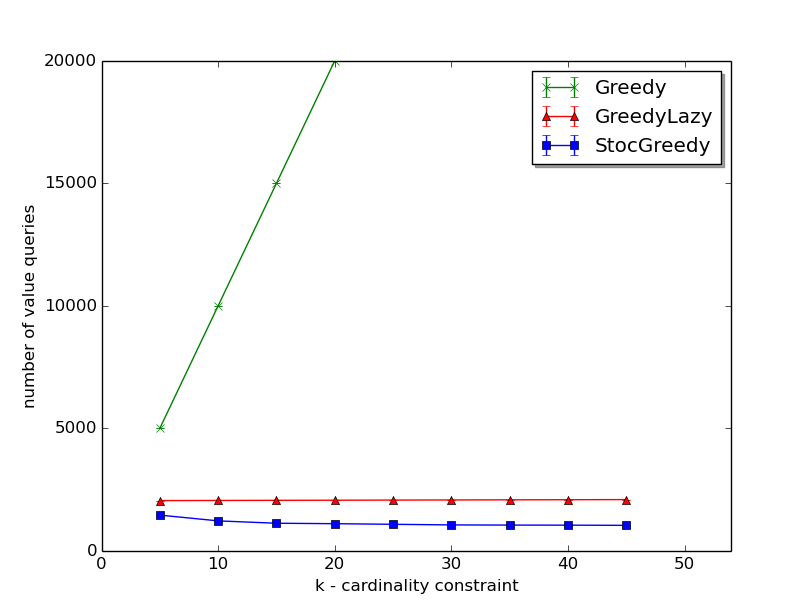
\includegraphics[width=0.5\textwidth]{figures/value-queries.png}
    \caption{Efficiency, measured by number of value queries being used}
    \label{fig:greedy-efficiency}
\end{figure}

\begin{figure}[h]
    \centering
    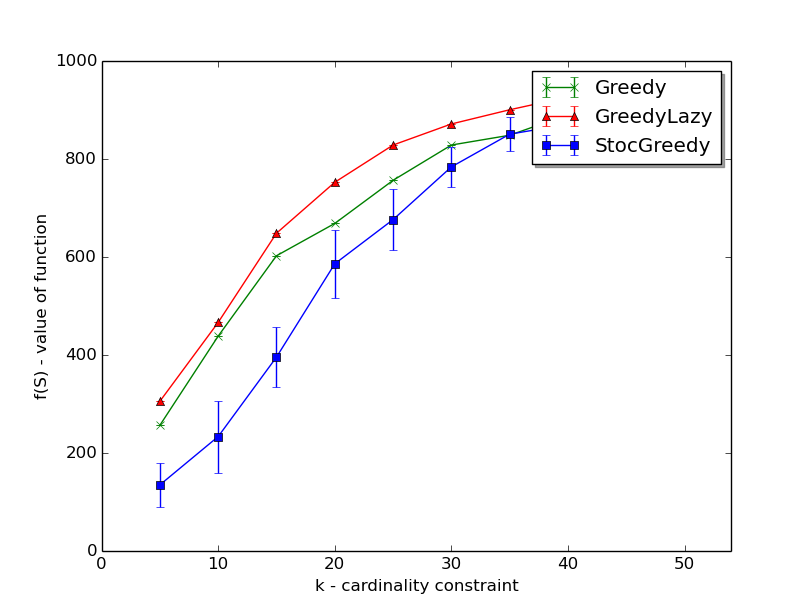
\includegraphics[width=0.5\textwidth]{figures/func-values.png}
    \caption{Quality of Returned Solutions}
    \label{fig:quality-greedy}
\end{figure}



\section{Streaming Submodular Maximization}
\label{sec:streaming}
We compare three different streaming algorithms in the problem of monotone submodular maximization subject to cardinality constraint. In generally it is hard to compare those algorithms fairly because they are configured by different type of parameters. To address this issue, we fixed parameters so that all three algorithms consume roughly the same amount of time. We also compare them with  the standard greedy algorithm (here we call it \offline) and a streaming algorithm (called \baseline) that generates the solution by using random sampling (the notable reservoir sampling is being used internally).


\subsection{Streaming Algorithms}
\begin{itemize}
\item \sieveStream \cite{BMK+14} gives $(1/2 - \eps)$-approximation. See \ref{algo:sieveStream} for details.
\item \randomStream \cite{CGQ15} gives $\frac{1 - \eps}{2 + \eps}$-approximation. See \ref{algo:randomStream} for details.
\item \circuitStream \cite{V11,CGQ15} gives $1/4$-approximation. See \ref{algo:circuitStream} for details.
\end{itemize}
We also compare above three algorithms with \offline and \baseline as mentioned.
\begin{algorithm}[H]
\DontPrintSemicolon % Some LaTeX compilers require you to use \dontprintsemicolon instead
\KwIn{$V$ as data stream, $f$ a monotone submodular function, $k$ the size constraint, $\eps$ a parameter}
\KwOut{a set $S \subseteq V$}
$O = \{(1 + \eps)^i~|~i\in \bbZ\}$\;
\tcc*[h]{maintain the sets only for the necessary $v$'s lazily}\;
For each $v\in O, ~S_v \gets \emptyset$\;
$m \gets 0$\;

\For{each $e$ in the data stream} {
  m $\gets \max\{m, f(\{e\})\}$\;
  $O\gets \{(1 + \eps)^i~|~m \leq (1 + \eps)^i \leq 2\cdot k \cdot m\}$\;
  Delete all $S_v$ such that $v \in O$\;
  \For{$v \in O$}{
    \If{$\Delta(e|S_v) \geq \frac{v/2 - f(S_v)}{k - |S_v|}$ and $|S_v|<k$}{
      $S_v \gets S_v \cup \{e\}$\;
    }
  }
}
\Return{$\argmax_{S_v: v\in O}f(S_v)$}\;
\caption{\sieveStream for submodular maximization}
\label{algo:sieveStream}
\end{algorithm}

\begin{algorithm}[H]
\DontPrintSemicolon % Some LaTeX compilers require you to use \dontprintsemicolon instead
\KwIn{$V$ as data stream, $f$ a non-negative submodular function, $k$ the cardinality constraint, $\eps$ a parameter}
\KwOut{a set $S \subseteq V$}
$B\gets \emptyset, S\gets \emptyset$\;
\For{each $e$ in the data stream} {
  \If{$|S| < k$ and $\Delta(e|S) > \alpha$}{
    $B \gets B + e$\;
  }
  \If{$|B| > \frac{k}{\eps}$}{
    $e \gets $ uniformly random from $B$\;
    $B \gets B - e, S \gets S + e$\;
    \For{all $e'\in B$ s.t. $\Delta(e'|S)\leq \alpha$}{
      $B \gets B - e'$\;
    }
  }
}
$S' \gets$ offline algorithm on $B$\;
\Return{$\argmax_{A\in\{S, S'\}}f(A)$}\;
\caption{\randomStream for submodular maximization}
\label{algo:randomStream}
\end{algorithm}

\begin{algorithm}[H]
\DontPrintSemicolon % Some LaTeX compilers require you to use \dontprintsemicolon instead
\KwIn{$V$ as data stream, $f$ a monotone submodular function, $k$ is the cardinality constraint, $\gamma > 0$ is a parameter}
\KwOut{a set $S \subseteq V$}

\For{each $e$ in the data stream} {
  \If{$|S| < k$}{
    $S \gets S + e$\;
  }
  \Else{
    $e^* \gets \argmin_{e'\in S}f(\{e'\})$\;       
    \If{$f(\{e\}) \geq (1 + \gamma)\cdot f(\{e^*\})$}{
      $S \gets S \cup \{e\} \backslash \{e^*\}$\;
    }  
  }
}
\Return $S$\;
\caption{\circuitStream for  submodular maximization}
\label{algo:circuitStream}
\end{algorithm}



\section{Distributed Submodular Maximization}
\label{sec:distributed}

\section{Discussion and Conclusion}
\label{sec:conclude}



%----------- end -------------------------













\bibliographystyle{abbrv}
\bibliography{survey.bib}

%\newpage

%\appendix
%\input{appendix}


\end{document}


\section{Conclusion and Future Research}
\label{sec:conclusion}
We have shown some of the nice properties of submodular functions and how they can be applied to various areas. Submodular maximization has been studied for many years but there are still many open problems left. Less results are known in streaming and distributed submodular maximization while these two models are playing increasingly important roles in ``big data'' era. We list several open problems/directions for future research.

\begin{itemize}
\item We mentioned that {\sc Stochastic-Greedy} in \cite{MBK+15} uses only $O(|V|\log\frac{1}{\eps})$ number of value queries based on a sampling technique, but this method only works for cardinality constraint. Is it possible to design fast sampling-based algorithms for more general constraints (e.g. matroid)?
\item There are several algorithms proposed for streaming submodular maximization, but most of them assume value oracle, which, unfortunately is not realistic in streaming model. Often we need the whole ground set to calculate the value of a submodular function. In \cite{BMK+14}, the authors discussed how one can deal with composable submodular (i.e. $f(S) = \sum_{v\in V}f_v(S)$) function via sampling. Can we also obtain some results for non-composable submodular functions?
\item We note that the power of submodularity is not fully explored in the area of database, can we identify some problems that may have submodular formulations? 
\item It would be interesting to extend submodular maximization to Distributed Monitoring Model \cite{CMY11}.
\end{itemize}


\bibliographystyle{abbrv}
\bibliography{survey.bib}

%\newpage

%\appendix
%\input{appendix}


\end{document}
